\documentclass[CJK,aspectratio=43]{beamer}  %aspectratio控制页面的宽高比,16:9充满屏幕
\usepackage{xeCJK}
\usepackage{booktabs}
\usepackage{multirow}
\usepackage{amsmath}   % 数学公式排版
\usepackage{graphicx}  % 插入图片和图形
\usepackage{hyperref}  % 创建超链接和交互式文档
\usepackage{geometry}  % 设置页面布局和边距
\usepackage{babel}     % 多语言支持
\usepackage[utf8]{inputenc}   % 设置文本编码
\usepackage[T1]{fontenc}     % 设置字体编码
\usepackage{xcolor}    % 创建颜色和调整颜色
\usepackage{listings}  % 排版代码和程序清单
\usepackage{caption}
\captionsetup[table]{skip=5pt} % 设置表格标题与内容之间的间距
\captionsetup[figure]{skip=5pt} % 设置图片标题与内容之间的距离
\usepackage{appendix}
\setmainfont[Mapping=tex-text]{Times New Roman}%--------------------------------英文衬线字体
\setsansfont[Mapping=tex-text]{Arial}%------------------------------------英文无衬线字体
\setmonofont[Mapping=tex-text]{Courier New}%-------------------------------------英文等宽字体
\newfontfamily\Arial{Arial}
% 默认的数学公式较难看,使用serif可以使得公式的样式变为常用latex的公式样式 
\usefonttheme[onlymath]{serif} 
\usetheme{Frankfurt} %对应网站的行
\usecolortheme{whale} %对应网站的列
\setbeamertemplate{headline}[frame number]
\expandafter\def\expandafter\insertshorttitle\expandafter{%
	\insertshorttitle\hfill%
	\insertframenumber\,/\,\inserttotalframenumber}
\definecolor{uibred}  {HTML}{db3f3d}
\definecolor{uibblue} {HTML}{4ea0b7}
\definecolor{uibgreen}{HTML}{789a5b}
\definecolor{uibgray} {HTML}{d0cac2}
\definecolor{uiblink} {HTML}{00769E}
\setbeamercolor{block body} {bg = uibgray}
\setbeamercolor{block title}{fg = white,bg = uibred}
\setbeamertemplate{caption}[numbered]
\title[投资组合优化]{基于收益预测和CVaR约束的投资组合优化}
\author{袁靖松}
\institute{金融数学专题展示}
\centering
\date{2023.12}
\begin{document}
	% 一般第一页显示PPT标题以及作者信息
	\begin{frame}
		\titlepage
	\end{frame}
	\begin{frame}{Outline}
		\tableofcontents[currentsection,hideallsubsections]
	\end{frame}
\section{研究背景}
\subsection{改进期望收益}
	\begin{frame}{改进期望收益}
			\begin{itemize}
				\item Mean-Variance存在缺陷,模型建立在资产收益率服从正态分布等诸多限制性假设之上;均值作为期望收益与实际市场不符;低通滤波;不适于短期投资;
			\begin{figure}
				\centering
				\includegraphics[width=1.04\linewidth]{"pic/distribution of random six"}
				\caption{Distribution}
				\label{fig:distribution-of-random-stock}
			\end{figure}
			\end{itemize}
	\end{frame}
\subsection{改进风险度量}
	\begin{frame}{改进风险度量}
		\begin{enumerate}
			\item 使用方差度量风险
			\begin{itemize}
				\item 对异常值敏感,极端风险事件,会显著影响方差计算;
				\item 只关注收益率分布的前两矩,忽略分布的尾部;
			\end{itemize}
			\item 使用CVaR来度量风险损失
			\begin{itemize}
				\item 对异常值不敏感
				\item 不依赖分布假设
				\item 考虑分布的尾部,更好处理异常值
			\end{itemize}
			\item 结合机器学习方法与现代投资组合优化理论~\cite{Ma2020}
		\end{enumerate}
	\end{frame}
\section{理论模型}
\subsection{资产及收益率}
\begin{frame}{资产及收益率}
	\begin{itemize}
		\item $N$种资产
		\item \textbf{收益率矩阵} $N\times T$
		$$
		R=
		\begin{bmatrix}
			r_1^1 & r_1^2 & r_1^3 & ... & r_1^T\\
			r_2^1 & r_2^2 & r_2^3 & ... & r_2^T\\
			r_3^1 & r_3^2 & r_3^3 & ... & r_3^T\\
			... & ... & ... & ... & ...\\
			r_N^1 & r_N^2 & r_N^3 & ... & r_N^T\\
		\end{bmatrix}
		=
		\begin{bmatrix}
			R_1 & R_2 & R_3 &... & R_T
		\end{bmatrix}
		$$
		其中$R_t$为 $t$ 时期 $N$ 种资产的收益率矩阵;
		\item \textbf{权重矩阵} $N \times 1$
		$$
		w=\begin{bmatrix}
			w_1 & w_2 & w_3 & ... & w_N
		\end{bmatrix}^T
		$$
	\end{itemize}
	\end{frame}

\subsection{VaR及CVaR}
	\begin{frame}{VaR及CVaR}
	\begin{itemize}
		\item \textbf{价值损失函数}
		$$
		L(w,R)=-w^TR
		$$
		其中,$w\in W\subseteq R^N$,$W$为可行集;$R$为随机变量,密度函数为$P(R)$;
		\item $L(w,R)$是依赖于 $w$ 的随机变量,小于临界值 $\lambda$ 的概率为:
		$$
		\varphi(w,\lambda)=\int_{L(w,R)\leq\lambda}P(R)dR
		$$
		\item \textbf{置信水平}: $\alpha\in(0,1)$
		$$
		\text{VaR}:\lambda_{\alpha}(w)=\text{inf}\{\lambda\in R;\varphi(w,\lambda) \geq \alpha \}
		$$
		$$
		\text{CVaR}:\phi_{\alpha}(w)=E[L(w,R) \vert L(w,R) \geq VaR(w)]
		$$
		$$
		=\frac{1}{1-\alpha}\int_{L(w,R)\geq \lambda_{\alpha}(w)}L(w,R)P(R)dR
		$$
	\end{itemize}
	\end{frame}

\begin{frame}{CVaR计算}
	\begin{itemize}
		\item 利用Rockafellar和Uryasev同时计算$\text{VaR}$和$\text{CVaR}$的功能函数$F_{\alpha}(w,R)$有
		$$
		F_{\alpha}(w,\lambda)=\lambda+\frac{1}{1-\alpha}\int_{R\in R^N}[L(w,R)-\lambda]^{+}P(R)dR
		$$
		其中,$\lambda$即$\text{VaR}$值,$[0,x]^+=\text{max}(0,x)$
		\item Rockafellar 和 Uryasev 提出,当$P(R)$的解析式未知时,可以使用基于历史数据的情景分析法,产生情景矩阵,将多重积分转化为求和运算;
		\item 假设有$m$种情况,可以取$N$种债券$m$个时期的收益率~\cite{Rong2007}
		$$
		\widehat{F}_{\alpha}(w,R)=\lambda+\frac{1}{m(1-\alpha)}\sum_{t=1}^{m}[L(w,R_t)-\lambda]
		$$
	\end{itemize}
\end{frame}

\subsection{优化问题建模}
\begin{frame}{优化问题建模}
	\begin{enumerate}
	\item CVaR最小化
		\begin{itemize}	
			\item 目标函数(决策变量: $w$)  \\
			$$
			\text{min}_{w} \ \lambda+\frac{1}{m(1-\alpha)}\sum_{t=1}^{m}[-w^TR_t-\lambda]
			$$
			\item 约束条件 \\
			$$
			\text{s.t.} \ w^TI=1
			$$
			$$
			w \geq 0
			$$
		\end{itemize}
	\item 方差最小化
		\begin{itemize}	
			\item 目标函数(决策变量: $w$) \\
			$$
			\text{min}_{w} \ w^T\Sigma w
			$$
			\item 约束条件 \\
			$$
			\text{s.t.} \ w^TI=1
			$$
			$$
			w \geq 0
			$$
		\end{itemize}
	\end{enumerate}
\end{frame}

\section{数据实验}
\subsection{数据及因子}
\begin{frame}{数据及因子}
	\begin{enumerate}
		\item 历史数据
		\begin{itemize}
			\item 沪深300名单内股票及指数月度收益数据
			\item 时间范围2005.04(month85)至2021.12(month285)
		\end{itemize}
		\item 部分因子
		\begin{itemize}
			\item \textbf{财务因子:}利润能力、偿债能力、资产周转率、现金流;
			\item \textbf{成长因子:}营收增长、利润增长、现金流增长;
			\item \textbf{市场因子:}股价相关、市值因子、动量;
			\item \textbf{其他因子:}风险、交易量、评级、股东持股变化、技术指标;
		\end{itemize}
	\end{enumerate}
	\begin{table}[htbp]
		\centering
		\resizebox{\textwidth}{!}{%
		\begin{tabular}{|l|l|l|l|l|l|}
			\toprule
			\multicolumn{1}{|c|}{\textbf{财务因子}} & \multicolumn{1}{c|}{\textbf{成长因子}} & \multicolumn{1}{c|}{\textbf{市场因子}} & \multicolumn{1}{c|}{\textbf{风险因子}} & \multicolumn{1}{c|}{\textbf{技术指标}} & \multicolumn{1}{c|}{\textbf{其他因子}} \\
			\midrule
			ROE\_q & Sales\_G\_q & return\_1m & beta  & macd  & LN\_capital \\
			\midrule
			ROE\_ttm & Profit\_G\_q & return\_3m & std\_1m & dea   & HAlpha \\
			\midrule
			ROA\_q & OCF\_G\_q & return\_6m & std\_3m & dif   & grossprofitmargin\_q \\
			\bottomrule
		\end{tabular}%
		}
		\label{tab:factors}%
		\caption{Factors}
	\end{table}%
\end{frame}

\subsection{选股及预测}
\begin{frame}{选股及预测}
	\begin{enumerate}
	\item 打分法选股
	\begin{itemize}
		\item 线性回归模型拟合训练集数据
		\item 使用回归系数、信息系数、因子协方差法为因子分配权重
		\item 根据不同股票的因子,得到分数较高的股票
	\end{itemize}
	\item 预测测试集收益率
	\begin{itemize}
		\item 使用PCA进行因子合成(Number of components based on Kaiser Criterion: 16)
		\begin{figure}
			\centering
			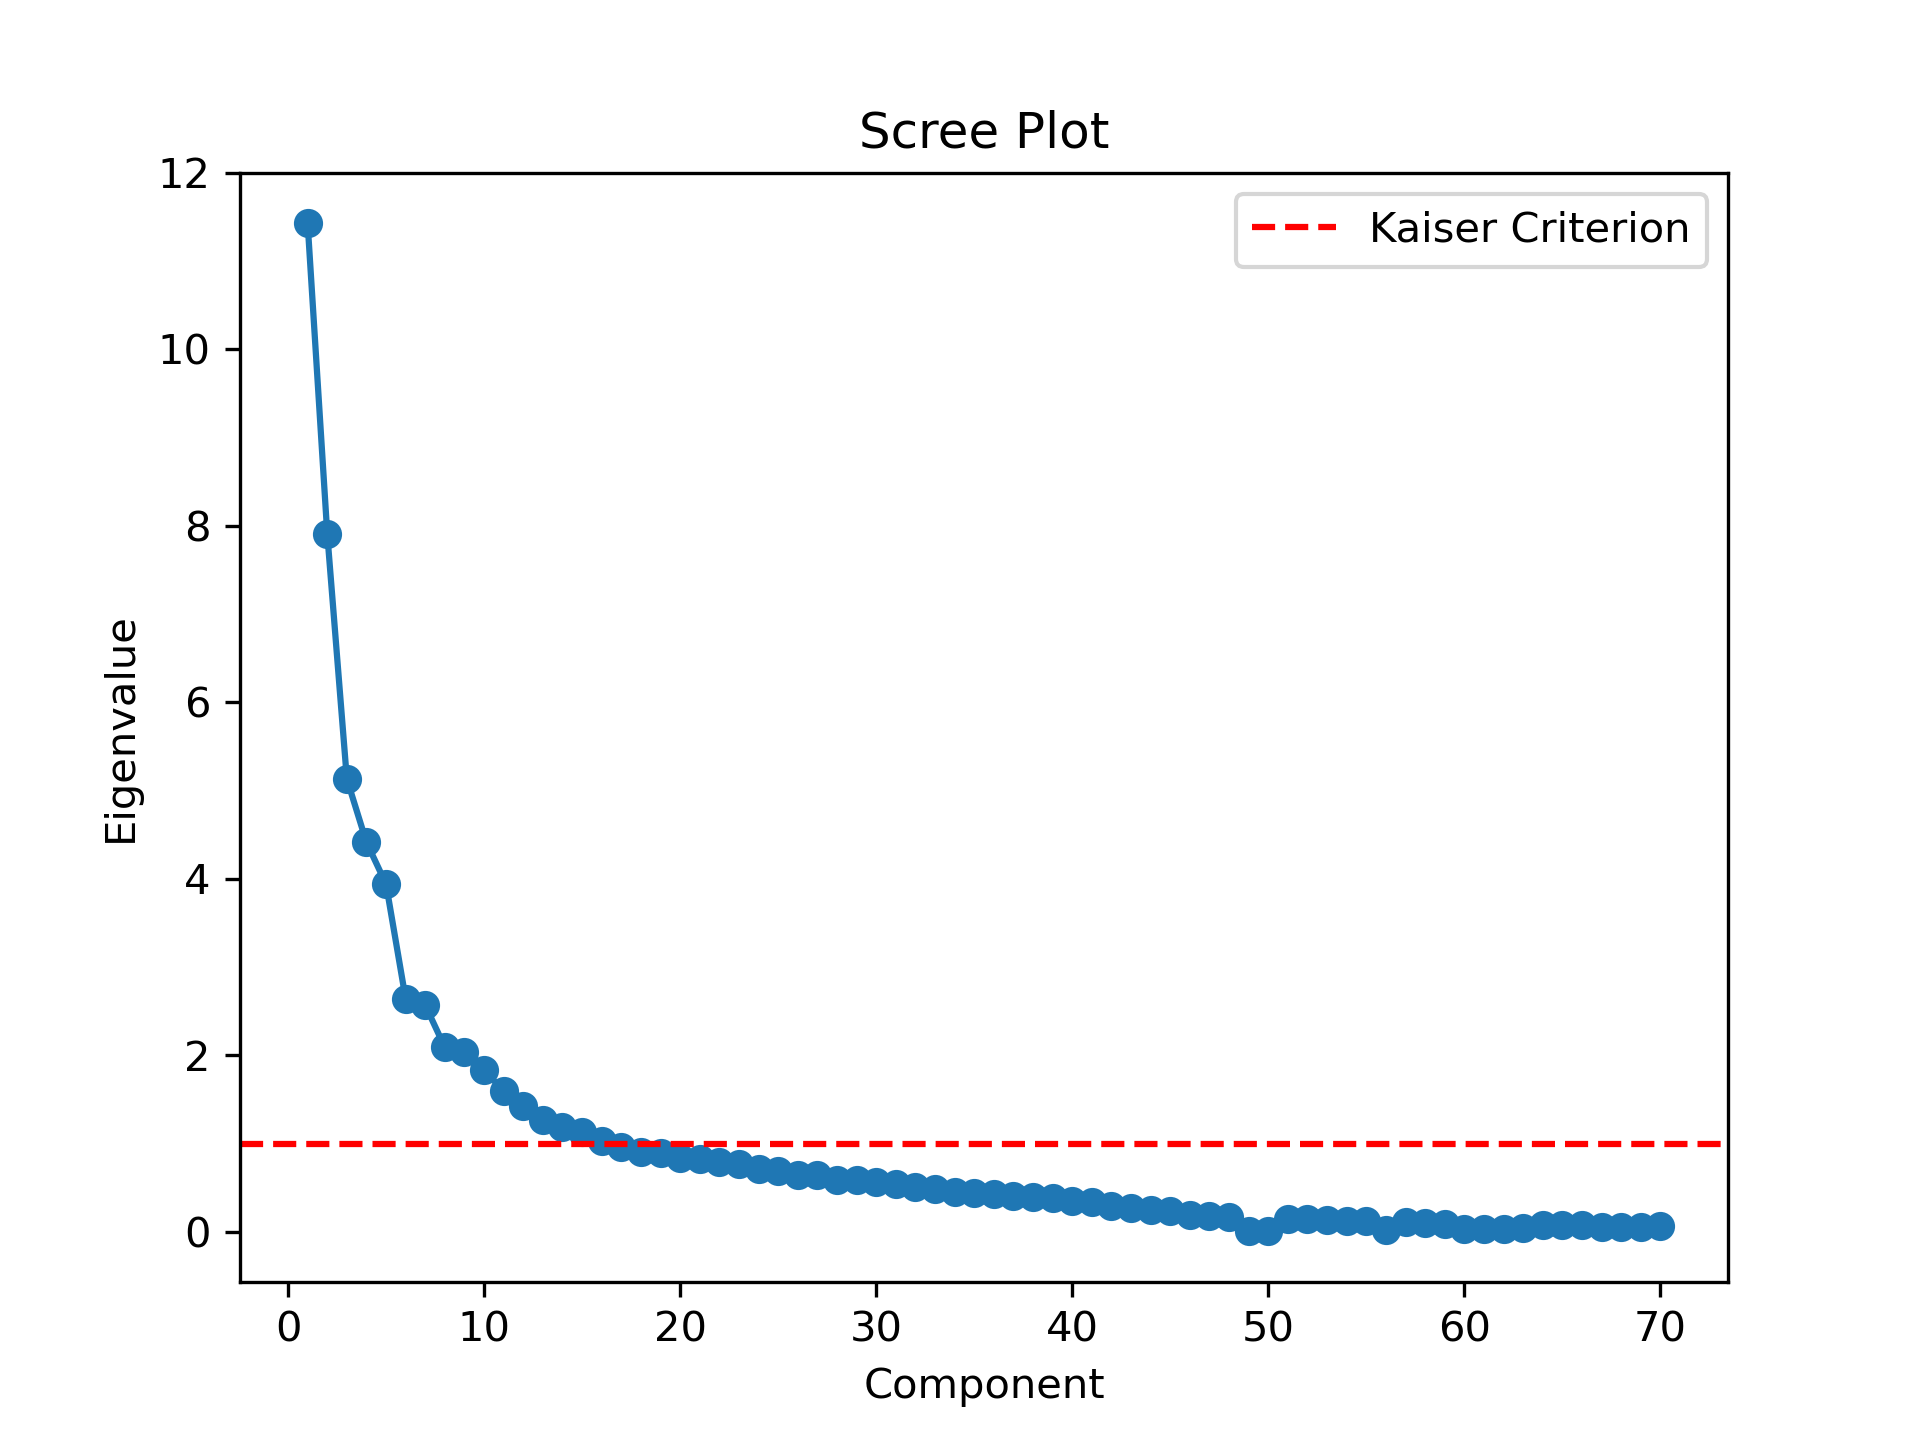
\includegraphics[width=0.58\linewidth]{pic/scree_plot}
			\caption{Scree Plot}
			\label{fig:screeplot}
		\end{figure}
		\item 拟合训练集的数据,预测测试集数据
	\end{itemize}
	\end{enumerate}
\end{frame}

\subsection{优化问题重构}
\begin{frame}{优化问题重构}
	\begin{enumerate}
		\item 决策变量为 $weights$
		\item 根据历史数据计算VaR
		\begin{itemize}
			\item 历史组合收益$ \text{Portfolio return} = Weights.T \times R $
			\item 置信水平为 $\alpha=99\%$
			\item 拟合组合收益的分布,取$1\%$处分位数为$VaR$值$=\lambda$
		\end{itemize}
		\item 加入预测数据计算CVaR(目标函数)
		\begin{itemize}
			\item 合并过去$40$个月历史数据,及预测的下$1$个月数据,形成新的数据集
			\item 代入$m$,$\alpha$,$L(w,R_t)=-Weights.T \times R_t$,$\lambda$到之前的解析式中
			$$
			\widehat{F}_{\alpha}(w,R)=\lambda+\frac{1}{m(1-\alpha)}\sum_{t=1}^{m}[L(w,R_t)-\lambda]
			$$
		\end{itemize}
	\end{enumerate}
\end{frame}

\subsection{Rolling Window}
\begin{frame}{Rolling Window}
	\begin{enumerate}
		\item 投资目标是短期投资
		\item 使用滚动训练的方法调整
		\begin{itemize}
			\item 训练集最少使用60个月的数据,最多不超过84个月
			\item 测试集是训练集之后的3个月
			\item 每3个月更新一次训练集及测试集
			\item 测试集每个月轮动一次,持仓时间实际上是1个月
			\item 测试集使用上一个月的因子数据,结合打分法选出下一个月的股票(避免未来函数)
		\end{itemize}
	\end{enumerate}
	\begin{figure}
		\centering
		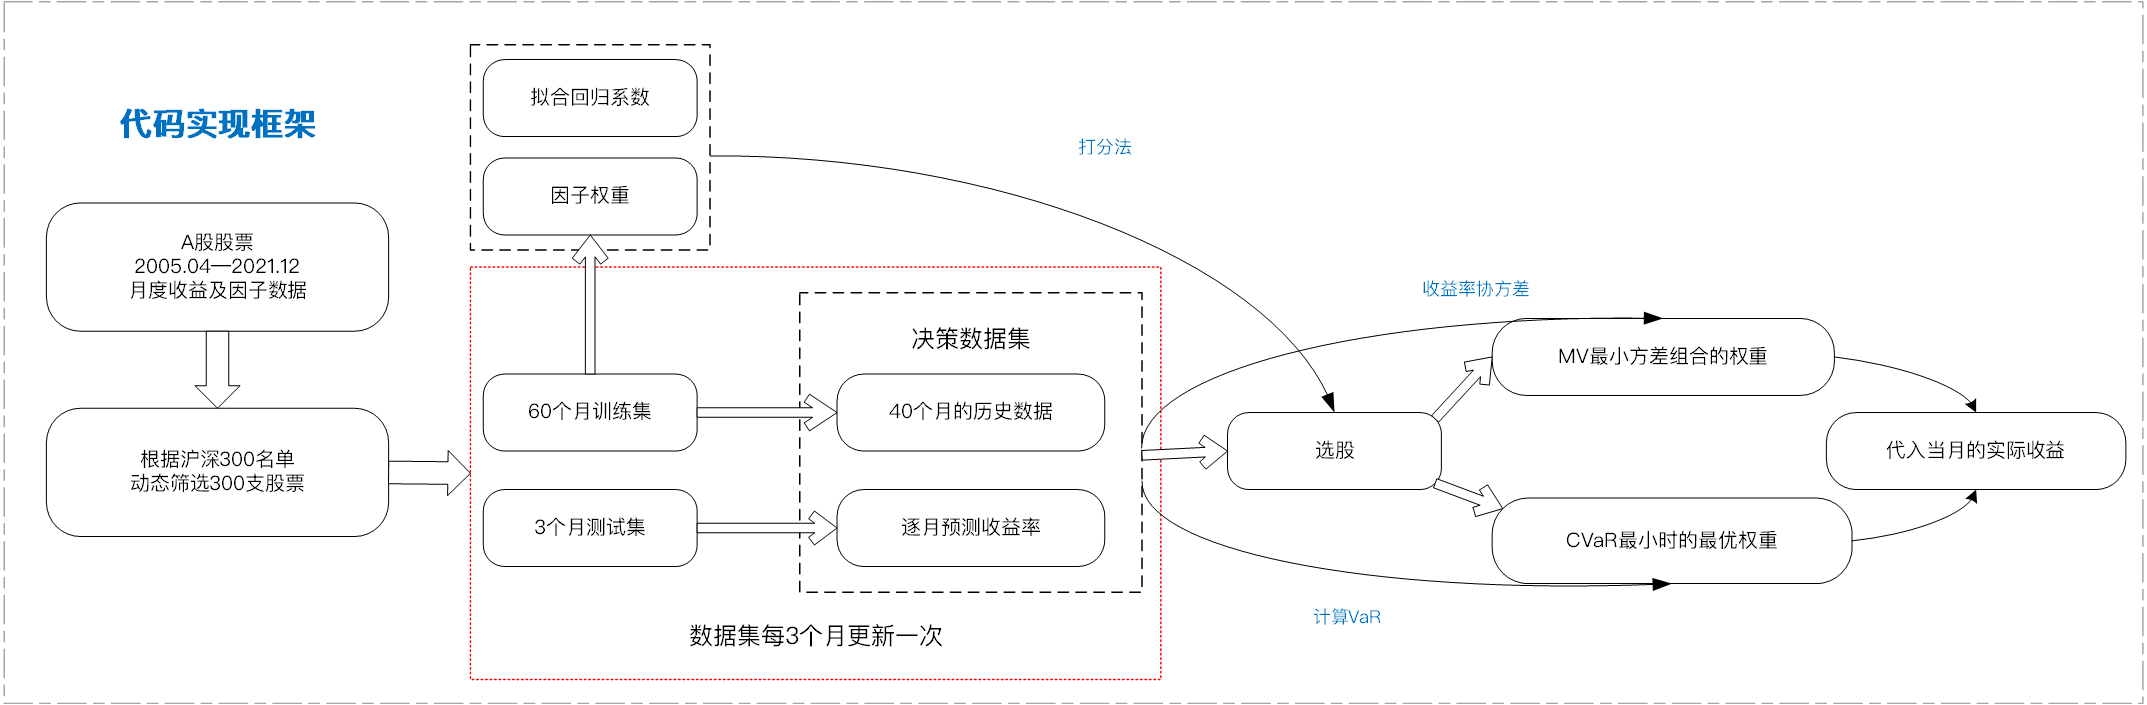
\includegraphics[width=0.95\linewidth]{pic/framework}
		\caption{Framework}
		\label{fig:framework}
	\end{figure}
\end{frame}

\subsection{回测}
\begin{frame}{回测思路}
	\begin{enumerate}
		\item 三种因子分配权重方法
		\begin{itemize}
			\item 按回归系数归一化配比
			\item 按信息系数归一化配比
			\item 按协方差矩阵的逆做配比
		\end{itemize}
		\item 两种最优权重求解方法
		\begin{itemize}
			\item Mean-Variance模型最小方差组合的权重
			\item 使CVaR值最小的权重
		\end{itemize}
		\item 与沪深300指数的收益对比
		\begin{itemize}
			\item 将最优权重分别代入当月的实际收益率,计算组合收益
			\item 将组合的收益与沪深300指数的收益对比
		\end{itemize}
	\end{enumerate}
\end{frame}

\subsection{Coef}
\begin{frame}{策略收益表现-Coef}
	\begin{itemize}
		\item 没有稳定明显地跑赢指数,CVaR策略小幅度优于MV策略
		\item 交易因子和财务因子,占较大权重
	\end{itemize}
	\begin{figure}
		\centering
		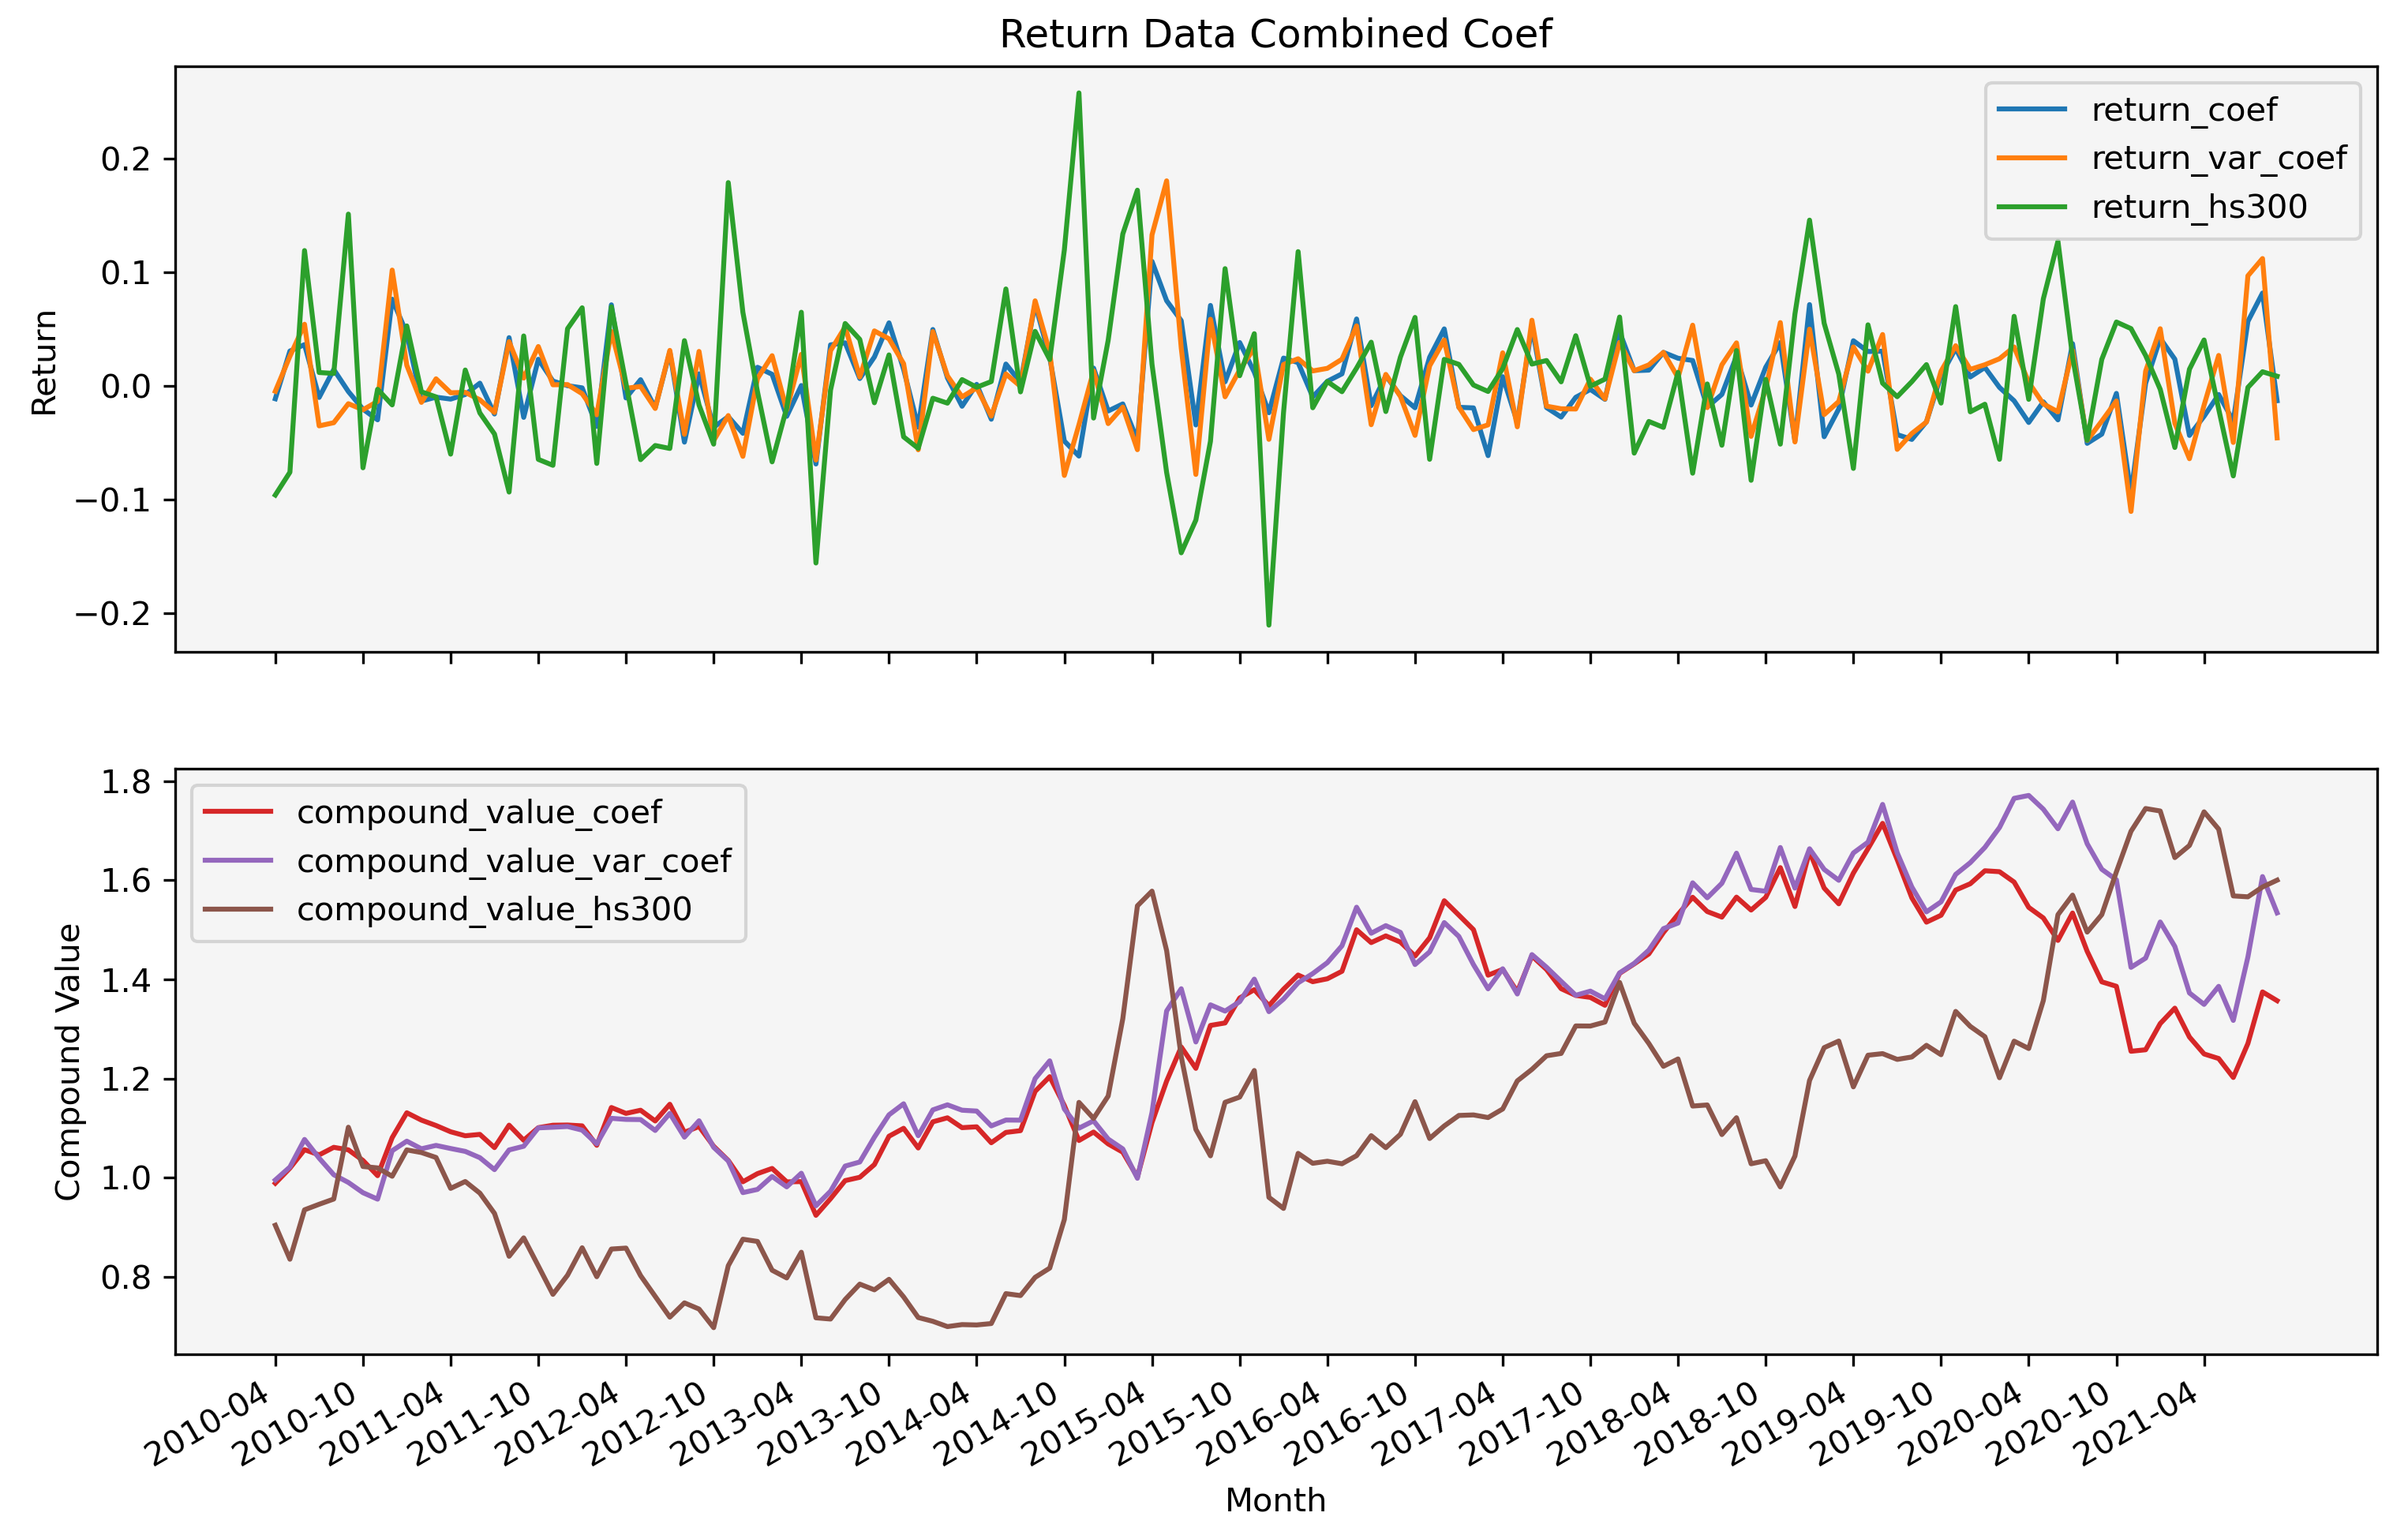
\includegraphics[width=0.85\linewidth]{pic/Coef}
		\caption{Return and Compound Value}
		\label{fig:coef}
	\end{figure}
\end{frame}

\begin{frame}{策略回撤-Coef}
	\begin{itemize}
		\item 两种策略最大回撤在 $20\%-30\%$,总体上回撤幅度低于指数
		\item 大幅回撤发生在2020年5月份之后
	\end{itemize}
	\begin{figure}
		\centering
		\includegraphics[width=1\linewidth]{"pic/Drawdown_Comparison_Coef"}
		\caption{Drawdown Comparison Coef}
		\label{fig:coefdramdown}
	\end{figure}
\end{frame}

\subsection{IC}
\begin{frame}{策略收益表现-IC}
	\begin{itemize}
		\item 总体上完全可以跑赢指数,CVaR策略完全优于MV策略;
		\item 2015年股市异常波动,高杠杆场外配资是股市异常波动主要原因;2020年年初,选股策略失效,可能是受疫情影响;
	\end{itemize}
	\begin{figure}
		\centering
		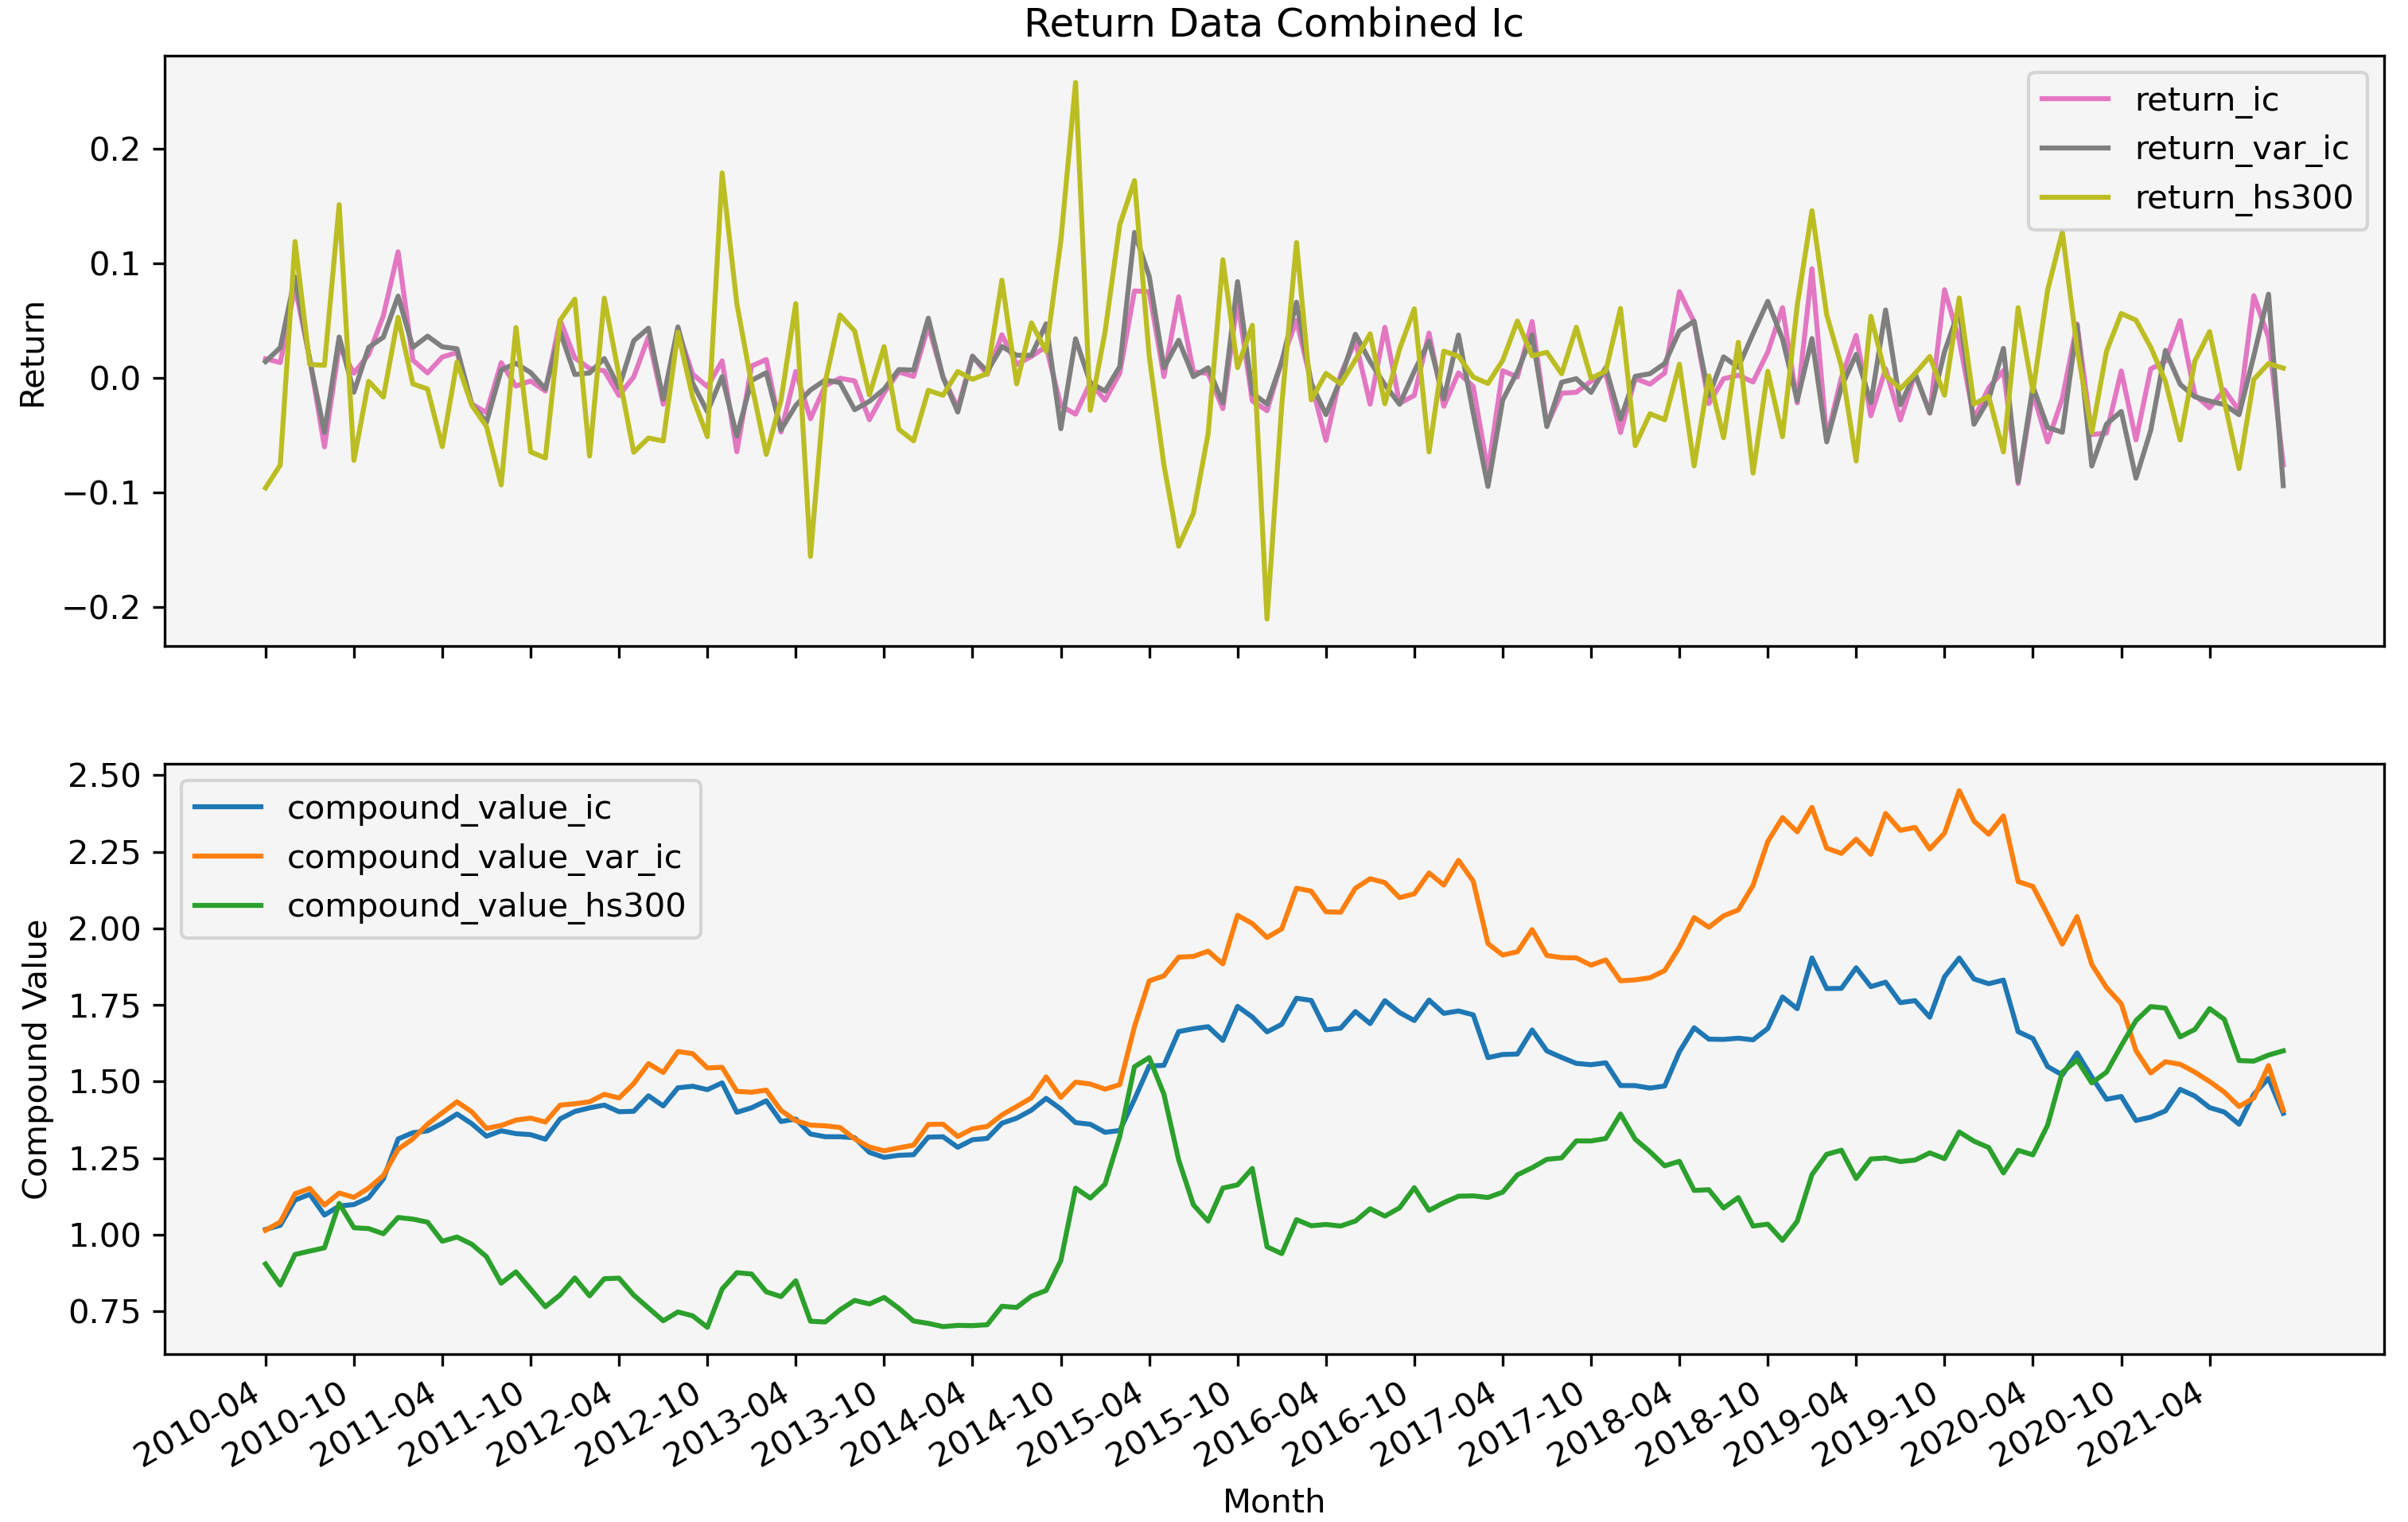
\includegraphics[width=0.79\linewidth]{pic/IC}
		\caption{Return and Compound Value}
		\label{fig:ic}
	\end{figure}
\end{frame}

\begin{frame}{策略回撤-IC}
	\begin{itemize}
		\item 在2019年末及2020年初,回撤幅度大幅增加
		\item 财务因子及股价因子,占较大权重
	\end{itemize}
	\begin{figure}
		\centering
		\includegraphics[width=1\linewidth]{"pic/Drawdown_Comparison_IC"}
		\caption{Drawdown Comparison IC}
		\label{fig:icdramdown}
	\end{figure}
\end{frame}

\subsection{Corr}
\begin{frame}{策略收益表现-Corr}
	\begin{itemize}
	\item 总体上大幅跑赢指数,CVaR策略逐步优于MV策略;
	\item 2015年异常波动;2019年年初异常波动,处于18年以来衰退末期,风险偏好回升,估值修复;
	\end{itemize}
	\begin{figure}
		\centering
		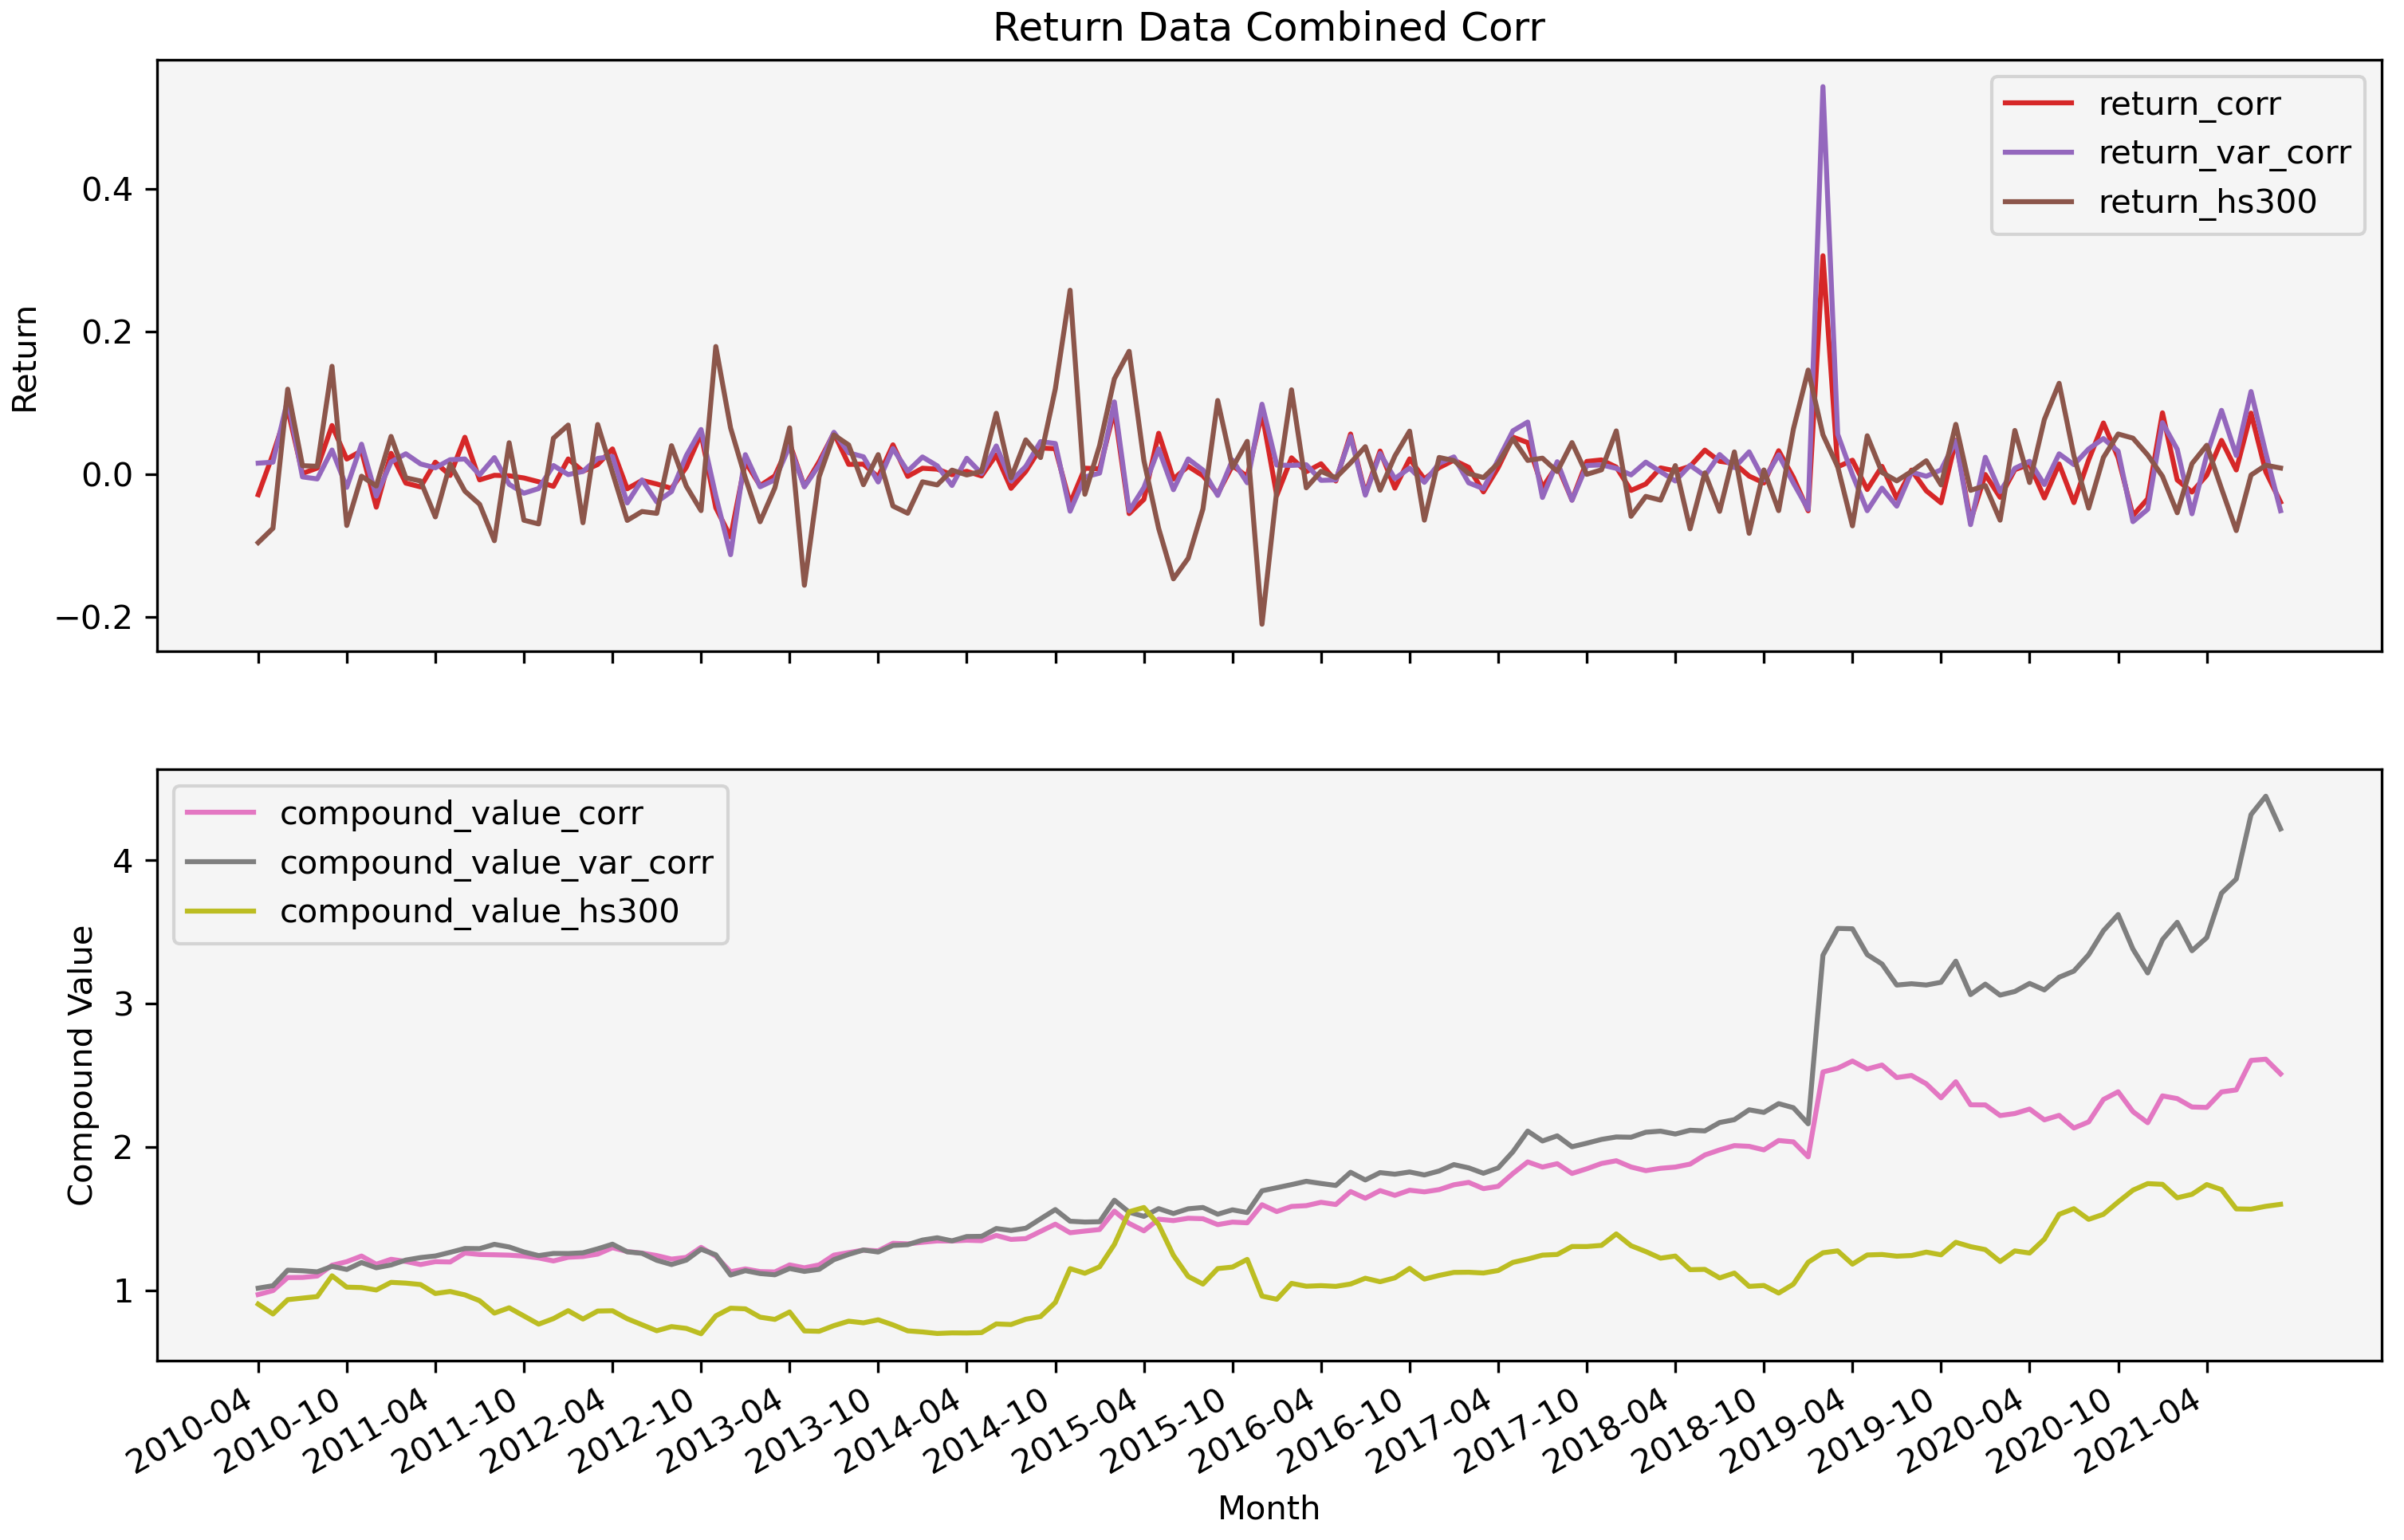
\includegraphics[width=0.79\linewidth]{pic/Corr}
		\caption{Return and Compound Value}
		\label{fig:corr}
	\end{figure}
\end{frame}

\begin{frame}{策略回撤-Corr}
	\begin{itemize}
		\item 总体上回撤幅度较小
		\item 股价及增长率因子占比为主,重视技术及情绪因子
		\item 疫情之后,传统的成长,动量等因子逐渐失效,估值,盈利,杠杆,非线性市值等因子表现突出
	\end{itemize}
	\begin{figure}
		\centering
		\includegraphics[width=1\linewidth]{"pic/Drawdown_Comparison_Corr"}
		\caption{Drawdown Comparison Corr}
		\label{fig:corrdramdown}
	\end{figure}
\end{frame}

\subsection{策略对比}
\begin{frame}{策略对比}
	\begin{itemize}
		\item CVaR策略基本优于MV策略,使用Corr方法选股+CVaR策略最优
		\item 10年期平均年化收益率 $15\%$
	\end{itemize}
	\begin{table}[htbp]
		\centering
		\resizebox{\textwidth}{!}{%
	    \begin{tabular}{|c|c|c|c|c|c|}
		\toprule
		\textbf{策略} & \textbf{最大回撤} & \textbf{夏普比率} & \textbf{信息比率} & \textbf{年化收益率} & \textbf{收益回撤比} \\
		\midrule
		Coef  & 29.901\% & 1.272 & -0.556 & 3.450\% & 11.538\% \\
		\midrule
		CVaR\_coef & 26.713\% & 1.510 & -0.309 & 4.867\% & 18.218\% \\
		\midrule
		Ic    & 28.526\% & 1.345 & -0.526 & 3.739\% & 13.108\% \\
		\midrule
		CVaR\_ic & 42.263\% & 1.395 & -0.484 & 4.025\% & 9.524\% \\
		\midrule
		Corr  & 17.969\% & 2.884 & 0.396 & 9.346\% & 52.009\% \\
		\midrule
		CVaR\_Corr & 16.723\% & 3.256 & 1.149 & 15.199\% & 90.889\% \\
		\midrule
		hs300 & 40.558\% & 1.336 & 0.000 & 6.845\% & 16.877\% \\
		\bottomrule
		\end{tabular}%
		}
		\caption{Strategy Comparison}
		\label{tab:compar}%
	\end{table}%
\end{frame}

\section{结论与不足}
\subsection{结论}
\begin{frame}{小结}
	\begin{enumerate}
	\item CVaR策略具有一定可行性
		\begin{itemize}
			\item 投资组合的权重决策,基本优于MV最小方差策略
			\item CVaR对损失风险更加敏感,投资组合的波动性更小
			\item 一定程度避免了人为模型设定误差和参数估计误差
			\item 同时获取超额收益的能力具有一定保障
		\end{itemize}
	\item CVaR策略的有效性受到诸多条件的影响
		\begin{itemize}
			\item 数据集划分、轮动周期
			\item 因子的数量及有效性
			\item 选股方法及选股数量
		\end{itemize}
	\end{enumerate}
\end{frame}

\subsection{不足}
\begin{frame}{不足}
	\begin{enumerate}
		\item 数据量小
		\begin{itemize}
			\item 只筛选出了沪深300的股票,整体的数据量较低
			\item 需要较多的历史数据才能拟合的比较精准
			\item 但历史数据的有效样本略微不足
			\item 月度数据,策略实效性较低
		\end{itemize}
			\item  历史数据选取时段缺乏标准(40个月)
		\begin{itemize}
			\item 过去时段过短,样本量少,反映尾部分布特征的样本较少
			\item 过去时段过长,样本量过多,收益率分布函数可能变化,无法反映先期收益率的分布特征
		\end{itemize}
		\item  没有考虑投资者观点
		\begin{itemize}
			\item 只考虑了风险指标
			\item 缺少对资产预期收益率的观点
			\item 只适合极端风险厌恶的投资者
			\item 理想的模型应该是权衡收益与风险的
		\end{itemize}
	\end{enumerate}
\end{frame}

\subsection{改进}
\begin{frame}{针对CVaR策略的改进方向}
	\begin{enumerate}
		\item 改进目标函数的估计方法
		\begin{itemize}
			\item $F_{\alpha}(w,\lambda)=\lambda+\frac{1}{1-\alpha}\int_{R\in R^N}[L(w,R)-\lambda]^{+}P(R)dR$
			\item 目标函数中包含极大值函数,是非光滑凸规划问题
			\item 考虑使用非参数核估计方法~\cite{Huang2014}
		\end{itemize}
		\item 改进约束条件
		\begin{itemize}
			\item 考虑交易成本
			\item 加入投资者观点,如定价误差参数、预期收益率等 $w^TR\geq \pi$
			\item 梯度计算公式+迫近束求解~\cite{Tong2021}
			\item 假设一种分布,如非对称-Laplace分布~\cite{Huang2022}
		\end{itemize}
		\item  改进代码实现方法
		\begin{itemize}
			\item 尝试更多ML/DNN方法选股及预测
			\item 改进滚动及调仓周期
			\item 改进因子配比方法
			\item 使用更高频数据
		\end{itemize}
	\end{enumerate}
\end{frame}

% 附录部分
\appendix
\section{因子权重}
\begin{frame}{因子权重}
	\begin{enumerate}
		\item 三种方法对应的因子权重
		\begin{table}[htbp]
			\centering
			\resizebox{\textwidth}{!}{%
			\begin{tabular}{|c|c|c|c|c|c|}
				\toprule
				\multicolumn{2}{|c|}{\textbf{Coef}} & \multicolumn{2}{c|}{\textbf{IC}} & \multicolumn{2}{c|}{\textbf{Corr}} \\
				\midrule
				\textbf{Factors} & \textbf{Weights} & \textbf{Factors} & \textbf{Weights} & \textbf{Factors} & \textbf{Weights} \\
				\midrule
				turn\_6m & 0.11  & EP    & 0.07  & EP    & 0.18 \\
				\midrule
				exp\_wgt\_return\_12m & 0.06  & EPcut & 0.06  & EPcut & 0.14 \\
				\midrule
				turn\_12m & 0.05  & ROE\_ttm & 0.06  & BP    & 0.10 \\
				\midrule
				bias\_turn\_6m & 0.04  & Profit\_G\_q & 0.06  & SP    & 0.09 \\
				\midrule
				exp\_wgt\_return\_1m & 0.03  & ROE\_q & 0.05  & NCFP  & 0.07 \\
				\midrule
				turn\_3m & 0.03  & OCFP  & 0.05  & OCFP  & 0.07 \\
				\midrule
				exp\_wgt\_return\_6m & 0.03  & ROE\_G\_q & 0.04  & DP    & 0.06 \\
				\midrule
				return\_1m & 0.03  & SP    & 0.04  & G/PE  & 0.06 \\
				\midrule
				std\_6m & 0.03  & DP    & 0.04  & Sales\_G\_q & 0.06 \\
				\midrule
				std\_1m & 0.03  & ROA\_ttm & 0.03  & Profit\_G\_q & 0.05 \\
				\bottomrule
			\end{tabular}%
			}
			\caption{Weights of Factors}
			\label{tab:top factors}%
		\end{table}%
	\end{enumerate}
\end{frame}

\section{参考文献}
\begin{frame}[t, allowframebreaks]
	\frametitle{参考文献}
	\bibliographystyle{plain}
	\bibliography{references.bib}
	\vfill
	\begin{center}
		\Huge\textbf{Thank You!}
	\end{center}
	\vfill
\end{frame}

\end{document}